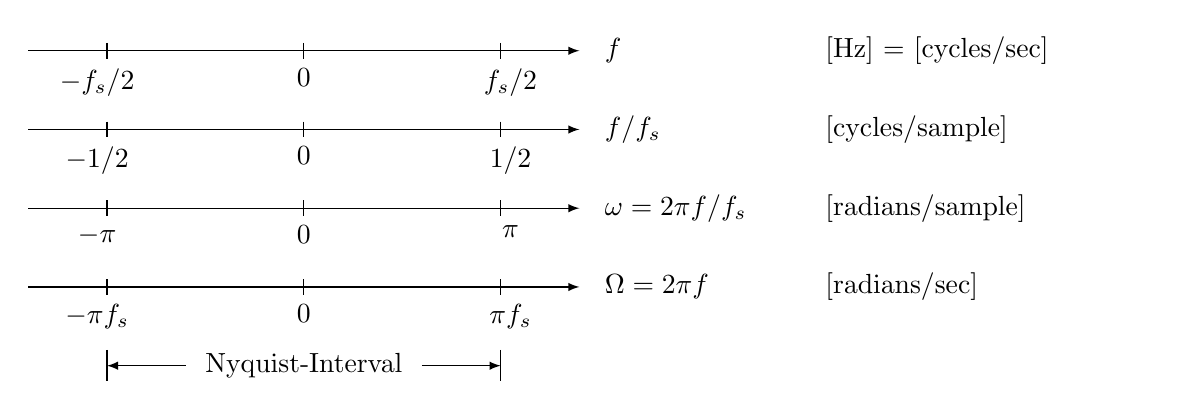
\begin{tikzpicture}
	\draw[-latex] (0,0) -- ++(7,0)
		node[midway, below={0.1cm}] {0}
		node[very near start, below={0.1cm}] {$-\pi f_s$}
		node[very near end, below={0.1cm}] {$\pi f_s$}
		node[at end, right={0.2cm}] {$\Omega = 2 \pi f$}
		node[at end, right={3cm}, text width=4cm] {[radians/sec]};
	\draw[-latex] (0,1) -- ++(7,0)
		node[midway, below={0.1cm}] {0}
		node[very near start, below={0.1cm}] {$-\pi$}
		node[very near end, below={0.1cm}] {$\pi$}
		node[at end, right={0.2cm}] {$\omega = 2 \pi f/f_s$}
	    node[at end, right={3cm}, text width=4cm] {[radians/sample]};
	\draw[-latex] (0,2) -- ++(7,0)
		node[midway, below={0.1cm}] {0}
		node[very near start, below={0.1cm}] {$-1/2$}
		node[very near end, below={0.1cm}] {$1/2$}
		node[at end, right={0.2cm}] {$f/f_s$}
		node[at end, right={3cm}, text width=4cm] {[cycles/sample]};
	\draw[-latex] (0,3) -- ++(7,0)
		node[midway, below={0.1cm}] {0}
		node[very near start, below={0.1cm}] {$-f_s/2$}
		node[very near end, below={0.1cm}] {$f_s/2$}
		node[at end, right={0.2cm}] {$f$}
		node[at end, right={3cm}, text width=4cm] {[Hz] = [cycles/sec]};
	% Markierungen
	\draw (1,0.1) -- +(0,-0.2)
		(3.5,0.1) -- +(0,-0.2)
		(6,0.1) -- +(0,-0.2);
	\draw (1,1.1) -- +(0,-0.2)
		(3.5,1.1) -- +(0,-0.2)
		(6,1.1) -- +(0,-0.2);
	\draw (1,2.1) -- +(0,-0.2)
		(3.5,2.1) -- +(0,-0.2)
		(6,2.1) -- +(0,-0.2);
	\draw (1,3.1) -- +(0,-0.2)
		(3.5,3.1) -- +(0,-0.2)
		(6,3.1) -- +(0,-0.2);
	% Anmerkung Nyquist Interval
	\draw (1,-0.8) -- +(0,-0.4)
		(6,-0.8) -- +(0,-0.4);
	\draw[-latex] (2,-1) -- +(-1,0);
	\draw[-latex] (5,-1) -- +(1,0);
	\node at(3.5, -1) {Nyquist-Interval};
\end{tikzpicture}